\documentclass{article}


% if you need to pass options to natbib, use, e.g.:
%     \PassOptionsToPackage{numbers, compress}{natbib}
% before loading neurips_2023


% ready for submission
\usepackage{neurips_2023}


% to compile a preprint version, e.g., for submission to arXiv, add add the
% [preprint] option:
%     \usepackage[preprint]{neurips_2023}


% to compile a camera-ready version, add the [final] option, e.g.:
%     \usepackage[final]{neurips_2023}


% to avoid loading the natbib package, add option nonatbib:
%    \usepackage[nonatbib]{neurips_2023}


\usepackage[utf8]{inputenc} % allow utf-8 input
\usepackage[T1]{fontenc}    % use 8-bit T1 fonts
\usepackage{hyperref}       % hyperlinks
\usepackage{url}            % simple URL typesetting
\usepackage{booktabs}       % professional-quality tables
\usepackage{amsfonts}       % blackboard math symbols
\usepackage{nicefrac}       % compact symbols for 1/2, etc.
\usepackage{microtype}      % microtypography
\usepackage{xcolor}         % colors


\title{Formatting Instructions For NeurIPS 2023}


% The \author macro works with any number of authors. There are two commands
% used to separate the names and addresses of multiple authors: \And and \AND.
%
% Using \And between authors leaves it to LaTeX to determine where to break the
% lines. Using \AND forces a line break at that point. So, if LaTeX puts 3 of 4
% authors names on the first line, and the last on the second line, try using
% \AND instead of \And before the third author name.


\author{%
  David S.~Hippocampus\thanks{Use footnote for providing further information
    about author (webpage, alternative address)---\emph{not} for acknowledging
    funding agencies.} \\
  Department of Computer Science\\
  Cranberry-Lemon University\\
  Pittsburgh, PA 15213 \\
  \texttt{hippo@cs.cranberry-lemon.edu} \\
  % examples of more authors
  % \And
  % Coauthor \\
  % Affiliation \\
  % Address \\
  % \texttt{email} \\
  % \AND
  % Coauthor \\
  % Affiliation \\
  % Address \\
  % \texttt{email} \\
  % \And
  % Coauthor \\
  % Affiliation \\
  % Address \\
  % \texttt{email} \\
  % \And
  % Coauthor \\
  % Affiliation \\
  % Address \\
  % \texttt{email} \\
}


\begin{document}


\maketitle


\begin{abstract}
  Chloe

  The abstract paragraph should be indented \nicefrac{1}{2}~inch (3~picas) on
  both the left- and right-hand margins. Use 10~point type, with a vertical
  spacing (leading) of 11~points.  The word \textbf{Abstract} must be centered,
  bold, and in point size 12. Two line spaces precede the abstract. The abstract
  must be limited to one paragraph.

  A short description of your goals, task, model, and (for
the final report) results. The abstract should make the
motivations and the scope of your project clear so that
readers can decide whether they are interested in
reading your work.
\end{abstract}


\section{Introduction}
Gabriel

A description of the motivation behind your work, why
the task you chose is interesting/important, and a
summary of your (proposed) approach. The problem
that you want to solve should be clearly stated in the
introduction: especially the input and output of your
model and the format of the input and output. This
section should also make it clear why your deep
learning approach is reasonable for this problem.

\section{Background and related work}
Chloe

A summary of the background material that students of
CSC413 would not already be familiar with. A
description of related work done in the area, and how
your approach compares with theirs.

If your project builds on previous work, clearly
distinguish what they did from what your new
contribution is. Also, include a 1-2 sentence summary
of other closely related papers. We realize you might
not know about all related papers (or have time to
carefully read all related papers), and that's OK for this
project. Using bibtex is annoying at first, but Google
Scholar can give you the bibtex entries.

\section{Data}
Taha 

The dataset used in your model. Include any key
exploratory figures that will help readers evaluate the
difficulty of your problem and interpret the performance
of your model.

https://www.kaggle.com/datasets/mathurinache/math-dataset

TODO: Find another dataset with proofs/numerical data


\section{Model architecture}
Everyone

A description of your (proposed) model architecture.
Please propose an architecture during the proposal
phase, but it's okay to change your architecture. In the
final report, this section should have enough details to
reproduce the work, including all hyperparameters and 3 training settings that you used.

 
Selected model: PaLM2 \\
Google PaLM2 = transformers + modifications: https://arxiv.org/pdf/2204.02311

Attempt to combine this with PaLM2: \\
SympyGPT: Transformers for symbolic integration proofs: https://arxiv.org/html/2410.02666v1


Better with word problems?
Architecture: PaLM, GPT4: http://research.google/blog/minerva-solving-quantitative-reasoning-problems-with-language-models/

We could also combine the two models (unlikely but look into it):

Standard Transformers Architecture: https://arxiv.org/abs/1706.03762

\section{Model architecture figure}
Takia

A figure that helps show the overall model or idea. The
idea is to make your paper more accessible, especially
to readers who are starting by skimming your paper.
You must create a new figure, not just use someone
else's, even with attribution. Be careful that all figure
text are legible, and are approximately the same size
as the main text.

% \begin{figure}[hbtp]
%   \centering
%   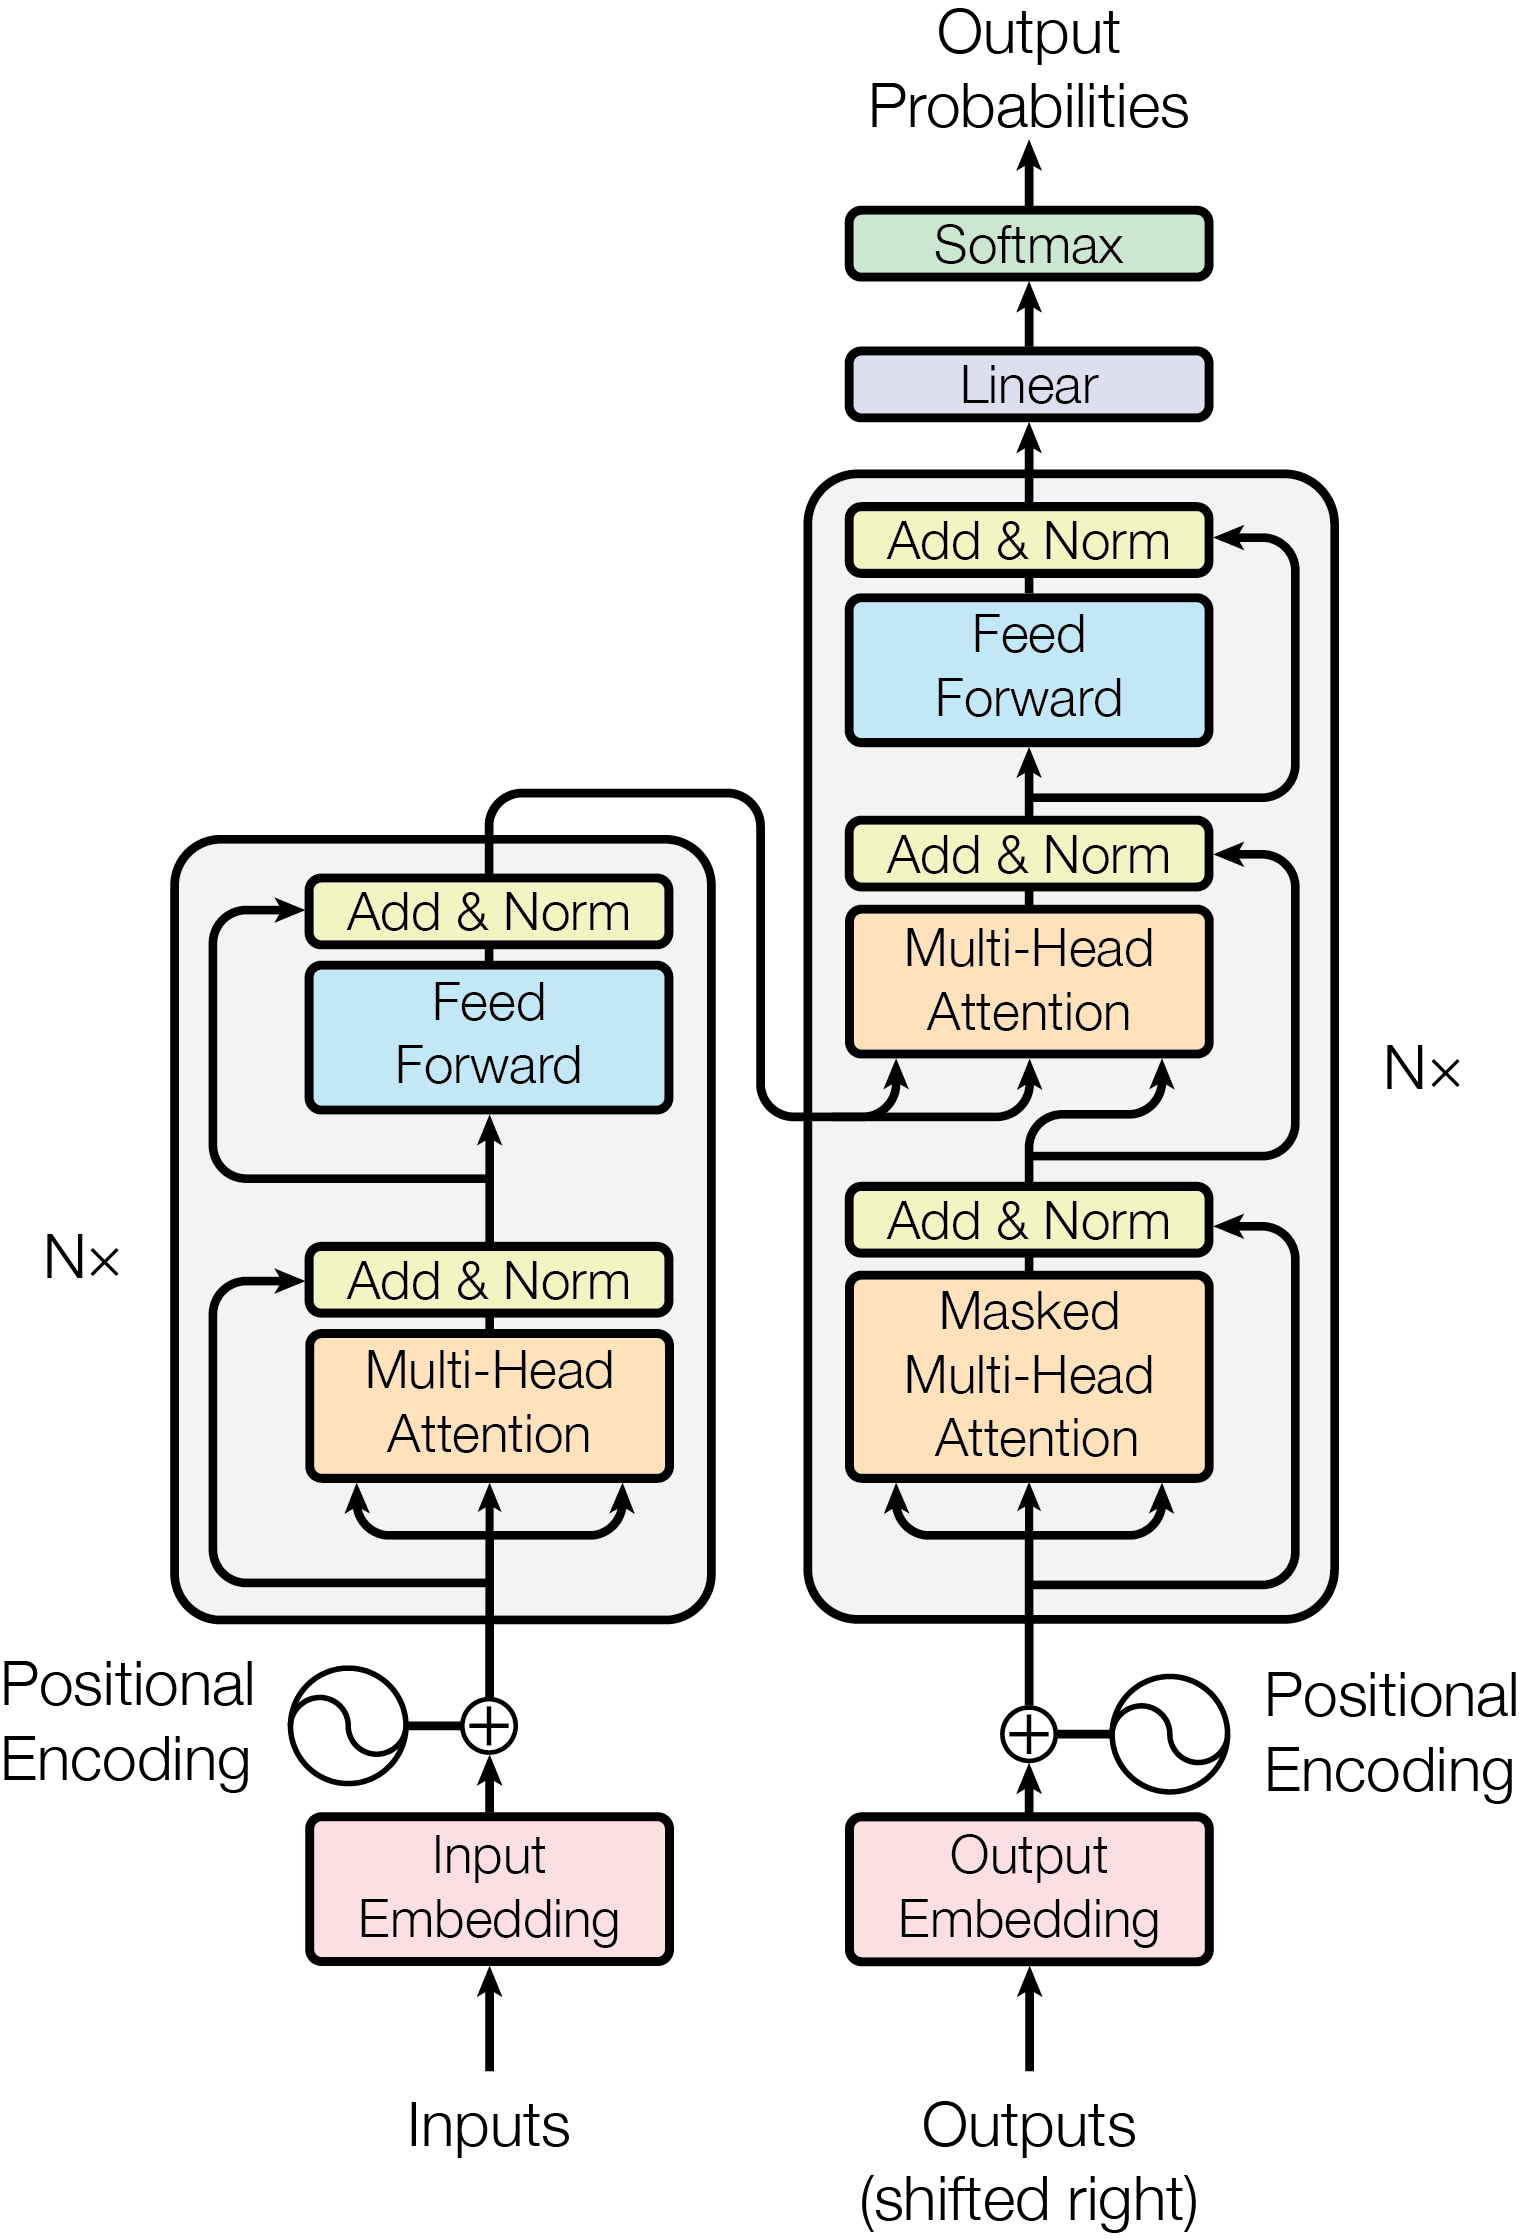
\includegraphics[scale=0.6]{./figures/ModalNet-21.png}
%   \caption{The Transformer - model architecture.}
%   \label{fig:model-arch}
% \end{figure}


% LEAVE FOR FINAL REPORT
% \section{Results}
% Describe the performance of your model, either
% quantitatively or (for generative models) qualitatively. To
% help interpret the model, compare your model with a
% baseline model. Qualitative evaluation is OK.


% LEAVE FOR FINAL REPORT
% \section{Discussion}
% Interpret the results of your model. If appropriate,
% compare the model performance with the baseline.
% Discuss other features that you notice about the model.


% LEAVE FOR FINAL REPORT
% \section{Limitations}
% Describe some settings in which we’d expect your
% approach to perform poorly, or where all existing
% models fail. Try to guess or explain why these
% limitations are the way they are. Give some examples
% of possible extensions, ways to address these
% limitations or open problems

\section{Ethical considerations}
Taha

Potential ethical issues posed by the use or misuse of
your model. Your report should transparently
communicate the known or anticipated consequences
of building and using machine learning models on this
task.

https://neurips.cc/public/EthicsGuidelines


\section{Work division}

A description of how the work will be divided between
the team members, and how the team members will be
working together (e.g. meet every week Tuesday 4-5
pm).

Chloe - Background and Related Work, Abstract, Model Architecture

Takia - Model Architecture Figure, Model Architecture

Gabriel - Introduction, Model Architecture

Taha - Data, Ethical Considerations, Model Architecture

The team will work on each part, and meet every weekend for additional discussions. 

% LEAVE FOR FINAL REPORT
% \section{Conclusion}

% A description of how the work will be divided between
% the team members, and how the team members will be
% working together (e.g. meet every week Tuesday 4-5
% pm).

\end{document}